\documentclass{beamer}


\usetheme{metropolis}

%\usecolortheme{beaver}


\usepackage{xltxtra}
\usepackage{polyglossia}

\RequirePackage[absolute,overlay]{textpos}


\setmainlanguage{russian}
\setotherlanguage{english}


\usepackage{amssymb, amsmath}



\setmainfont{PT Sans}
\setromanfont{PT Sans} 
\setsansfont{PT Sans} 
\setmonofont{PT Sans} 
 
\newfontfamily{\cyrillicfont}{PT Sans} 
\newfontfamily{\cyrillicfontrm}{PT Sans}
\newfontfamily{\cyrillicfonttt}{PT Sans}
\newfontfamily{\cyrillicfontsf}{PT Sans}
 


\setkeys{russian}{babelshorthands=true}






\addto\captionsrussian{%

  \renewcommand{\figurename}{Рис.}%

  \renewcommand{\tablename}{Табл.}%

}




\title{Введение в анализ данных}
%\date{\today}
%\author{Matthias Vogelgesang}
%\institute{Centre for Modern Beamer Themes}

\begin{document}

\maketitle



%\begin{frame}

%\begin{textblock*}{120mm}(15mm,15mm)
 
%\end{textblock*}  

%\end{frame}

\begin{frame}
Понятие интеллектуального анализа данных соответствует широко
распространенному термину Data Mining, который часто переводится как
добыча данных, глубинный анализ данных, извлечение знаний, раскопка
знаний в базах данных.
\end{frame}

\begin{frame}

Вот  популярные слова   из описания вакансий  специалиста Data Science: 
\it{
SQL, Python, R,  SAS, Hadoop, Java, 
optimization, C++, visualization, MATLAB,  Business Intelligence, 
distributed computation, 
machine learning, 
unstructured,
Hive.}


Видно, насколько разносторонней  (междисциплинарной)  должна быть эта квалификация с
точки зрения современного работодателя.   


\end{frame}


\begin{frame}

Data Mining -- мультидисциплинарная область, возникшая и развивающаяся на базе таких наук, 
как прикладная статистика, распознавание образов, искусственный интеллект, теория баз данных и др.

 Data Mining это процесс необходимый для  поддержки принятия решений, основанный на
поиске в данных скрытых закономерностей или аномалий.

\end{frame}
 


\section{Основы обработки данных и  основы алгоритмизации}

\subsection{Основы представления данных}

\begin{frame}

В широком понимании данные представляют собой факты, текст,
графики, картинки, звуки, аналоговые или цифровые видео-сегменты.
Данные могут быть получены в результате измерений, экспериментов,
арифметических и логических операций.

\end{frame}

\begin{frame}
Данные должны быть представлены в форме, пригодной для 
хранения, передачи и обработки. Иными словами, данные --
это необработанный материал, предоставляемый поставщиками данных и используемый
потребителями для формирования информации на основе данных.
\end{frame}

\begin{frame}
Набор данных  представляют в простом случае двухмерной таблицей, в которой 
строки это объекты, а столбцы это атрибуты или еще их называют измерения

Атрибут - свойство, характеризующее объект: цвет глаз человека,
температура воды и т.д. Атрибут также называют полем таблицы.
\end{frame}



\begin{frame}

\textbf{Адекватность информации } - это уровень соответствия образа, создаваемого с помощью информации, реальному объекту, процессу, явлению.
 
 От степени адекватности информации зависит правильность принятия решения.

Адекватность информации может выражаться в трех формах: синтаксической, семантической и прагматической.

\end{frame}

\begin{frame}{Синтаксическая адекватность}

\textbf{Синтаксическая адекватность} отображает формально-структурные характеристики информации, не затрагивая ее смыслового содержания. 
На синтаксическом уровне учитываются тип носителя и способ представления информации, 
скорость ее передачи и обработки, размеры кодов представления информации, 
надежность и точность преобразования этих кодов и т. д.

Информацию, рассматриваемую с таких позиций, обычно называют данными.

\end{frame}

\begin{frame}{Семантическая адекватность}

\textbf{Семантическая адекватность} определяет степень соответствия образа объекта самому объекту. 
Здесь учитывается смысловое содержание информации. На этом уровне анализируются сведения, отражаемые информацией, 
рассматриваются смысловые связи. 
Таким образом, семантическая адекватность проявляется при наличии единства информации и пользователя. 
Эта форма служит для формирования понятий и представлений, выявления смысла, содержания информации и ее обобщения.

\end{frame}

\begin{frame}{Прагматическая адекватность}

\textbf{Прагматическая адекватность} отражает соответствие информации цели управления, реализуемой на ее основе. 
Прагматические свойства информации проявляются при наличии единcтва информации, пользователя и цели управления. 
На этом уровне анализируются потребительские свойства информации, связанные с практическим использованием информации, 
с соответствием ее целевой функции деятельности системы.

\end{frame}

\begin{frame}{Информационный процесс}

\begin{small}

\begin{itemize}


  \item Поиск информации — это извлечение  информации  для сбора и хранения 

  \item Сбор информации предназначен для придания информации адекватности.  Для этого необходима обработка информации, то есть
   преобразование информации из одного вида в другой, осуществляемое по формальным правилам. 
 
  \item Хранение информации — это способ распространения информации в пространстве и времени в доступном виде. Другая цель это  многократное
   использование информация. 

  \item  Передача. В процессе передачи информации обязательно участвуют источник и приемник информации: первый передает информацию, второй ее получает. Между ними действует 
  канал передачи информации — канал связи. 
 
\end{itemize}

\end{small}

\end{frame}





\subsection{Типы данных:time-series, cross-section,  panel-data.} 


\begin{frame}{Типы данных:time-series} 

Временной ряд — совокупность наблюдений одного и того же показателя в различные моменты времени 
(обычно последовательные: дни, недели, месяцы, кварталы, годы и т.д.).

Показатели: цены акций, уровень безработицы, обменный курс евро/рубль и т.д. 
Характерной особенностью временных рядов является естественным образом зафиксированный порядок наблюдений. 


\end{frame}




\begin{frame}{Типы данных:cross-section}

''Перекрёстные данные'' — это тип данных, собранный путем наблюдения за многими объектами 
(такими как физические лица, фирмы, страны или регионы) в один и тот же период времени.

Для перекрестных данных (дословный перевод термина cross-sectional data, 
иногда он переводится как «пространственные данные» в противопоставление временным, или «временной срез») 
момент времени зафиксирован, и имеются наблюдения для различных однородных объектов (в этот момент). 
\end{frame}

\begin{frame}{Типы данных:panel-data} 

Панельные данные —  это набор наблюдений за некоторыми однородными объектами в различные моменты времени. 
Если объекты в разные моменты времени одни и те же, то панель называется сбалансированной 
(например, известны данные о потреблении 10 индивидов в течение 5 лет без пропусков),
 а если различаются — то несбалансированной (например, известны данные о потреблении 4 индивидов в течение 
 5 лет без пропусков, 5 индивидов в течение первых 4 лет и 1 индивида в течение последних 3 лет). 
 
\end{frame}


\begin{frame}{Групповая обработки данных} 
\begin{enumerate}
\item Описательная статиcтика 
\item Фильтрация 
\item Заполнение пропусков
\item Дубликаты и противоречия
\item Редактирование выбросов 
\item Спектральная обработка предназначена для очистки от шумовой составляющей и сглаживания рядов данных. Сглаживание необходимо в том случае, когда ряд данных оказывается неравномерным, содержит большое количество мелких структур, препятствующих исследованию более значительных объектов и закономерностей. 


\end{enumerate}




\end{frame}




\begin{frame}{Схема map-reduce} 
MapReduce предполагает, что oбработка данных происходит в 3 стадии:
\begin{enumerate}

\item  Стадия Map.
\item   Стадия Shuffle.
\item   Стадия Reduce.
\end{enumerate}

\end{frame}

\begin{frame}{Схема map-reduce. Лямбда-архитектура  } 

Лямбда-архитектура - это архитектура обработки данных основанная на  использовании схемы vap-, разработанная для обработки огромных объемов данных с использованием методов пакетной и потоковой обработки.
 Этот подход к архитектуре пытается сбалансировать задержку, пропускную способность и отказоустойчивость. Два представления представления могут быть объединены перед представлением. лямбда-архитектуры коррелирует с ростом больших данных, аналитикой в реальном времени и стремлением снизить задержки при уменьшении карты.

\end{frame}

\begin{frame}{Схема map-reduce. Стадия Map} 

    На этой стадии данные предобрабатываются при помощи функции map(), которую определяет пользователь. Работа этой стадии заключается в предобработке и фильтрации данных. Работа очень похожа на операцию map в функциональных языках программирования – пользовательская функция применяется к каждой входной записи.

Функция map() примененная к одной входной записи и выдаёт множество пар ключ-значение. Множество – т.е. может выдать только одну запись, может не выдать ничего, а может выдать несколько пар ключ-значение. Что будет находится в ключе и в значении – решать пользователю, но ключ – очень важная вещь, так как данные с одним ключом в будущем попадут в один экземпляр функции reduce.

\end{frame}

\begin{frame}{Схема map-reduce. Стадия shuffle и  reduce.} 


\begin{itemize}

\item   Стадия Shuffle. Проходит незаметно для пользователя. В этой стадии вывод функции map «разбирается по корзинам» – каждая корзина соответствует одному ключу вывода 
стадии map. В дальнейшем эти корзины послужат входом для reduce.


\item   Стадия Reduce. Каждая «корзина» со значениями, сформированная на стадии shuffle, попадает на вход функции reduce().

Функция reduce задаётся пользователем и вычисляет финальный результат для отдельной «корзины».
Множество всех значений, возвращённых функцией reduce(), является финальным результатом MapReduce-задачи. 

\end{itemize}

\end{frame}

\begin{frame}{Схема map-reduce}

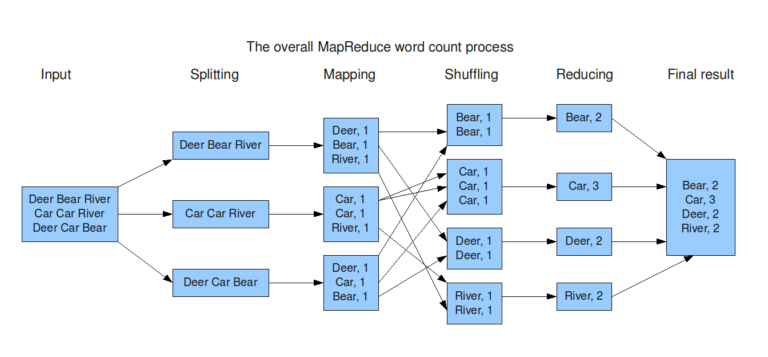
\includegraphics[scale=0.4]{ris_01.png}

$http://www.igfasouza.com/blog/$

\end{frame}




\section{ Существующие, наборы данных, визуализация модели классификации}

\begin{frame}{Существующие, наборы данных, визуализация}

Работа с «грязными» данными: редактирование, форматирование, 
удаление недопустимых значений и дубликатов. 
Агрегирование данных. Основные модели классификации

Рассматривать мы будем  программный продукт Orange3, позволяющий  интерактивно работать с данными.
Для знакомства выполним несколько заданий



\end{frame}

\begin{frame}{Работа с «грязными» данными}

Противоречивость информации;

Пропуски в данных;

Аномальные значения;

Шум;

Ошибки ввода данных. 

\end{frame}

\begin{frame}{Задание 1. Открыть файл}
  
  
  Виджет File считывает файл входных данных (таблица данных с экземплярами данных) и отправляет набор данных в свой выходной канал. История последних открытых файлов сохраняется в виджете. Виджет также включает в себя каталог с примерами наборов данных, которые предварительно установлены с Orange.

\end{frame}


\begin{frame}{Задание 2}

Нарисовать данные на двухмерной плоскости. Можно ставить отдельные точки данных или использовать 
кисть для рисования больших наборов данных.
Данные: новый набор данных, как нарисовано на графике
Виджет поддерживает создание нового набора данных путем визуального размещения 
точек данных на двухмерной плоскости. Точки данных могут быть размещены на плоскости 
индивидуально (Put) или в большем количестве с помощью кисти (Brush). 
Точки данных могут принадлежать классам, если данные предназначены для использования в контролируемом обучении.  

\end{frame}



\begin{frame}{Задание 3. Работа с грязными данными}

  
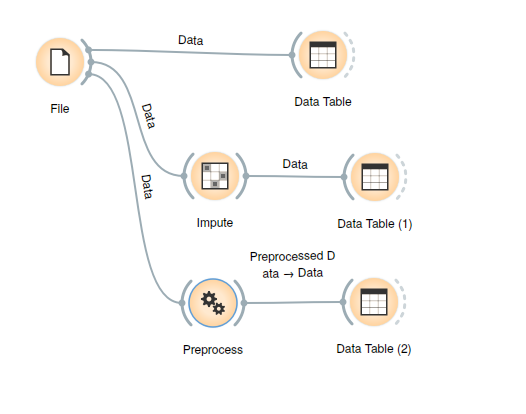
\includegraphics[scale=0.4]{task03_01.png}


\end{frame}


\begin{frame}{Задание 4. Визуализация}


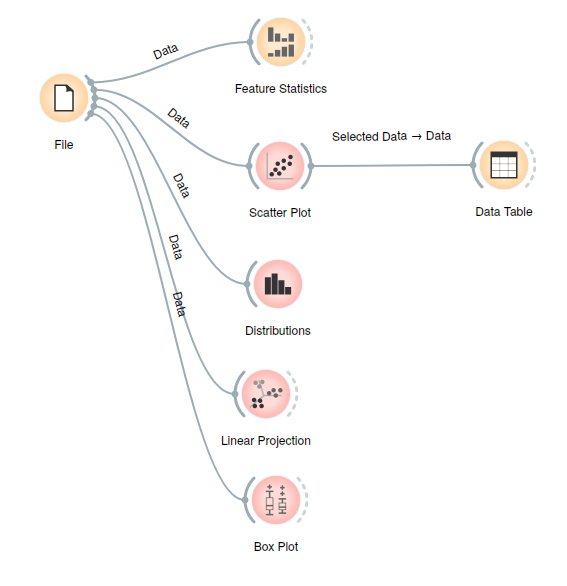
\includegraphics[scale=0.4]{task04_01.png}

\end{frame}



\begin{frame}{Агрегирование данных} 

Агрегирование  позволяет преобразовать группы наблюдений в наблюдения,
 содержащие агрегированную информацию по соответствующей группе, 
 и создавать новый, агрегированный, набор  данных Наблюдения агрегируются 
 на основе значений нуля или большего числа группирующих переменных. 
 Если группирующие переменные не заданы, то весь набор данных представляет 
 собой единую группу для агрегирования.

 Агрегация должна  содержать по одному наблюдению на каждую группу, определяемую группирующей переменной. 

\end{frame}



\begin{frame}{Агрегирование данных} 

Группирующие переменные. Наблюдения разбиваются на группы, на основании значений этих переменных. Каждая уникальная комбинация значений группирующих переменных определяет группу. 

Агрегируемые переменные. Для создания новых переменных используются исходные переменные с груповыми функциями.  



\end{frame}

\begin{frame}{Агрегирование данных} 

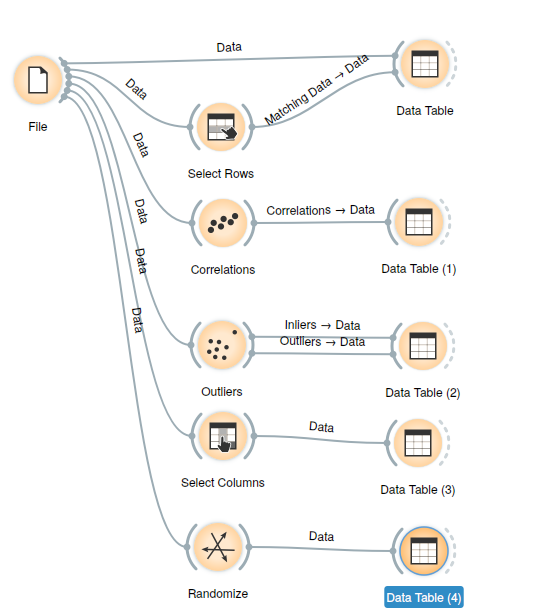
\includegraphics[scale=0.3]{task05_01.png}

\end{frame}






\begin{frame}{Методы классификации} 

Классификатор -  систематизированный перечень наименованных объектов, каждому из которых в соответствие дан уникальный код.  

В классификаторах применяется три метода классификации: иерархический, фасетный и дескрипторный. 
Выбор между этими тремя методами зависит от особенностей конкретной предметной области. 
Существуют следующие требования для выбранной системы классификации:

\begin{itemize}
 \item достаточная eмкость и необходимая полнота, которые гарантируют охват всех объектов классификации в заданных границах;
 \item оправданная глубина;
 \item обеспечение возможности решения комплекса задач различного уровня;
 \item возможность расширения множества классифицируемых объектов и внесения необходимых изменений в структуры классификации;
 \item обеспечение возможности сопряжения с другими классификациями однородных объектов;
 \item обеспечение простоты ведения классификатора.

\end{itemize}
 

\end{frame}

\begin{frame}{Методы классификации: Иерархический метод} 

Иерархическим методом классификации понимается метод, при котором  объекты делятся  
на вложенные или подчиненные подмножества, движение идет в сторону конкретизации 
объектов. При этом основанием деления служит  одно из свойств объекта. 
Совокупность получившихся группировок при этом образует иерархическую древовидную структуру, узлами которого являются группировки.
\end{frame}

\begin{frame}{Методы классификации: Иерархический метод} 
Выбор последовательности признаков зависит, прежде всего, от характера информации. 
При построении классификации выбор последовательности признаков зависит 
от вероятности обращения к тому или иному признаку. 
При этом наиболее вероятным обращениям должны соответствовать высшие уровни классификации.
\end{frame}

\begin{frame}{Методы классификации: Иерархический метод} 
Требования к классификатору, построенному на иерархическом методе классификации: Классификационные группировки, расположенные на одной ступени классификатора, не должны 
пересекаться, то есть не должны включать в себя аналогичных понятий. На каждой ступени классификатора для разделения вышестоящей группировки должен использоваться только 
один признак. Сумма подмножества всегда должна давать делимое множество объектов; не должна оставаться часть объектов, не вошедших в состав классификационной группировки.
\end{frame}

\begin{frame}{Методы классификации: Иерархический метод} 
Основными преимуществами иерархического метода является большая информационная ёмкость, 
традиционность и привычность применения, возможность создания для объектов классификации
мнемонических кодов, несущих смысловую нагрузку.

Значительным недостатком иерархической классификации является слабая гибкость структуры, 
обусловленная фиксированным основанием деления и заранее установленным порядком следования, не допускающим включение новых объектов и классификационных группировок.  


\end{frame}






\begin{frame}{Методы классификации: Фасетная классификация}

Фасетный метод классификации подразумевает параллельное разделение множества объектов на независимые 
классификационные группировки. При этом не предполагается жёсткой классификационной структуры и заранее построенных конечных группировок. 
Классификационные группировки образуются путём комбинации значений, взятых из соответствующих фасетов.
 Последовательность расположения фасетов при образовании классификационной группировки задается ''фасетной формулой''.
  Количество фасетных формул определяется возможными сочетаниями признаков.
\end{frame}

\begin{frame}{Методы классификации: Фасетная классификация} 
К классификатору, построенному на фасетном методе классификации, предъявляются следующие требования:
\begin{enumerate}
  \item Должен соблюдаться принцип непересекаемости фасета, то есть состав признаков одного фасета не должен повторяться в других фасетах этого же класса;
  \item В состав классификатора должны быть включены только такие фасеты и признаки, которые необходимы для решения конкретных задач.
\end{enumerate}

\end{frame}

\begin{frame}{Методы классификации: Фасетная классификация} 
Основным ''преимуществом'' классификации с использованием фасетного метода является гибкость структуры её построения.
 Изменения в любом из фасетов не оказывают существенного влияния на все остальные. 
При фасетной классификации появляется возможность объектов и осуществления
 информационного поиска по любому сочетанию фасетов.

''Недостатками'' фасетного метода классификации являются неполное использование 
ёмкости, нетрадиционность и иногда сложность применения.


\end{frame}


\begin{frame}{Методы классификации: Дескрипторная классификация}

Для организации поиска информации, для ведения тезаурусов (словарей) эффективно используется дескрипторная (описательная) система классификации,
 язык которой приближается к естественному языку описания информационных объектов:   
\end{frame}
 
 \begin{frame}{Методы классификации: Дескрипторная классификация}
 
\begin{enumerate}
\item  отбирается совокупность ключевых слов или словосочетаний, описывающих определенную предметную область или совокупность однородных объектов.
\item  выбранные ключевые слова и словосочетания подвергаются нормализации, т.е. из совокупности синонимов выбирается один или несколько наиболее употребимых;
\item  создается словарь дескрипторов, т.е. словарь ключевых слов и словосочетаний, отобранных в результате процедуры нормализации.
\item  между дескрипторами устанавливаются связи, которые позволяют расширить область поиска информации.

\end{enumerate}

\end{frame}


\begin{frame}{Методы классификации: Дескрипторная классификация}

Связи могут быть трех видов:

\begin{enumerate}

\item  синонимические, указывающие на некоторую совокупность ключевых слов как 
синонимов («студент – учащийся – обучаемый»);
\item  родовидовые, отображающие включение некоторого класса объектов в более 
представительный класс («университет – факультет – кафедра»);
\item  ассоциативные, соединяющие дескрипторы, обладающие общими свойствами 
(«студент – экзамен – профессор – аудитория»).

\end{enumerate}

\end{frame}






\section{Объекты и признаки. Типы шкал. Типы задач: классификация, регрессия, прогнозирование, ранжирование.}


\begin{frame}

Абсолютные статистические величины. Относительные статистические величины. 
Описательная статистика: медиана, среднее, разница применении и их трактовки. Объекты и признаки. 
Типы шкал: бинарные, номинальные, порядковые, количественные. Типы задач: классификация, регрессия, прогнозирование, ранжирование.
\end{frame}

\begin{frame}{Абсолютные статистические величины} 

Изучая массовые общественные явления, статистика в своих выводах опирается на числовые данные, полученные в конкретных условиях места и времени. Результаты статистического наблюдения регистрируются прежде всего в форме первичных абсолютных величин. . Абсолютная величина отражает уровень развития явления.

В статистике все абсолютные величины являются именованными, измеряются в конкретных единицах и, в отличие от математического понятия абсолютной величины, могут быть как положительными, так и отрицательными (убытки, убыль, потери и т.п.).

\end{frame}

\begin{frame}{Относительные статистические величины.}

Относительная величина в статистике – это обобщающий показатель, который дает числовую меру соотношения двух сопоставляемых абсолютных величин. Так как многие абсолютные величины взаимосвязаны, то и относительные величины одного типа в ряде случаев могут определяться через относительные величины другого типа.

\end{frame}

\begin{frame}{Относительные статистические величины.}
Основное условие правильного расчета относительной величины – сопоставимость сравниваемых показателей и наличие реальных связей между изучаемыми явлениями. Таким образом, по способу получения относительные показатели – всегда величины производные, определяемые в форме коэффициентов, процентов, промилле, продецимилле и т.п. Однако нужно помнить, что этим безразмерным по форме показателям может быть, в сущности, приписана конкретная, и иногда довольно сложная, единица измерения. 


\end{frame}


\begin{frame}{Номинальная}

Объекты классифицированы, классам присвоены
(наименований) словесные наименования или условные номера -
коды. То, что номер одного класса больше или
меньше другого, еще ничего не говорит о свойствах объектов, относящихся к этим классам, за
исключением того, что они различаются.

\end{frame}


\begin{frame}{Порядковая}

Объекты классифицированы, а классы обозначены номерами (закодированы). Значения чисел, 
присваиваемые классам, качественно отражают степень выраженности определенных свойств предметов, 
принадлежащих этим классам. То есть большим
значениям кодов классов соответствует и большая
степень выраженности измеряемого свойства, на
основании чего классы можно ранжировать.

\end{frame}

\begin{frame}{Интервальная}

 Существует единица измерения, при помощи которой классы можно не только 
 упорядочить, но и
приписать им числа так, чтобы равные разности
чисел присвоенных классам, отражали равные различия 
в количествах измеряемых свойств. Нулевая
точка интервальной шкалы произвольна (условна)
и не указывает на отсутствие свойства.


  
\end{frame}

\begin{frame}{Типы задач: классификация, регрессия, прогнозирование, ранжирование}

\begin{itemize}
  \item  Классификация
  \item  Регрессионный анализ
  \item  Прогнозирование
  \item  Ранжирование
  \item  Кластеризация 
\end{itemize}

\end{frame}
 

\begin{frame}{Типы задач: классификация}


Классификация — один из разделов машинного обучения, посвященный решению 
следующей задачи. Имеется множество объектов (ситуаций), разделённых некоторым образом на классы. 
Задано конечное множество объектов, для которых известно, к каким классам они относятся. 
Это множество называется обучающей выборкой. Классовая принадлежность остальных 
объектов не известна. Требуется построить алгоритм, способный классифицировать 
произвольный объект из исходного множества.

Классифицировать объект — значит, указать номер (или наименование класса), к которому относится данный объект.

Классификация объекта — номер или наименование класса, выдаваемый алгоритмом 
классификации в результате его применения к данному конкретному объекту.
\end{frame}
 

\begin{frame}{Типы задач: классификация}

В математической статистике задачи классификации называются также задачами дискриминантного анализа.

В машинном обучении задача классификации относится к разделу обучения с учителем. 
Существует также обучение без учителя, когда разделение объектов обучающей выборки на классы не задаётся, 
и требуется классифицировать объекты только на основе их сходства друг с другом. 
В этом случае принято говорить о задачах кластеризации или таксономии, и классы называть, 
соответственно, кластерами или таксонами. 



\end{frame}


\begin{frame}{Типы задач:  регрессия}

Регрессионный анализ — метод моделирования измеряемых данных и исследования их свойств. 
Данные состоят из пар значений зависимой переменной (переменной отклика) и независимой 
переменной (объясняющей переменной). 
Регрессионная модель есть функция независимой переменной и параметров с добавленной случайной переменной. 
Параметры модели настраиваются таким образом, что модель наилучшим образом приближает данные.
Критерием качества приближения (целевой функцией) обычно является среднеквадратичная ошибка: сумма квадратов разности значений модели и зависимой переменной для всех значений независимой переменной в качестве аргумента. 
 
\end{frame}




\begin{frame}{Типы задач: прогнозирование}

Прогноз — это процесс или результат предсказания тех или иных фактов, событий, 
явлений, величин, которые станут известны лишь в будущем по 
отношению к моменту времени, в котором создается прогноз. Под прогнозом также иногда понимают 
модель будущего события, явления и т. п.

Прогнозирование — это процесс (часто основанный на научном исследовании) по расчету 
прогноза или разработке прогнозной модели.


\end{frame}

\begin{frame}{Типы задач: прогнозирование}
В узком смысле под прогнозированием понимают предсказание будущих значений временного 
ряда на основе его значений в прошлом, и, возможно, дополнительной информации. 
Такую дополнительную информацию представляют влияющие на ситуацию внешние факторы. 
Например, для прогнозирования временного ряд спроса на какой-либо товар 
это могут быть предложения замещающих товаров, для экспортных грузоперевозок - 
таможенные пошлины и курс доллара, для цен акций — политические решения и т. д. 


\end{frame}


\begin{frame}{Типы задач: ранжирование}

Задачи заключающиеся в подборе ранжирующей модели по обучающей выборке, 
состоящей из множества списков и заданных частичных порядков на элементах
 внутри каждого списка. Частичный порядок обычно задаётся путём указания оценки для каждого элемента 
 (например, «релевантен» или «не релевантен»; возможно использование и более, чем двух градаций). 
 Цель ранжирующей модели — наилучшим образом (в некотором смысле) приблизить и обобщить способ
  ранжирования в обучающей выборке на новые данные.

\end{frame}


\section{Показатели вариации. Линейные и нелинейные модели регрессии.}


\begin{frame}
Показатели вариации: дисперсия, стандартное квадратичное отклонение.
Перцентили, метод расчета, применение, трактовка.
Асимметрия, эксцесс, их применение и трактовка. Понятие выброса. 
Снижение волатильности через монотонное преобразование.
 Линейные модели регрессии и классификации.
  Метод наименьших квадратов. 
  Полиномиальная регрессия. 
  Понятие причинности, корреляция. 
  Получение и трактовка коэффициентов.
\end{frame}


\begin{frame}{Показатели вариации: дисперсия, стандартное квадратичное отклонение.}

$$S=\sqrt{\frac{1}{n}\sum_{i=1}^n\left(x_i-\bar{x}\right)^2}$$

Дисперсию определяют как квадрат стандартного квадратичного отклонения
 $S^2$ -дисперсия

\end{frame}


\begin{frame}{Показатели вариации: дисперсия, стандартное квадратичное отклонение.}


Дисперсия 

$$D[X] = (X -M[X])^2$$
 
 $M[X]$ - Математическое ожидание
 
 
 Среднеквадратическое отклонение определяется как квадратный корень из дисперсия случайной величины:
 
 $$\sigma = \sqrt{D[X]}$$

\end{frame}

\begin{frame}{Показатели вариации: $r^2$}

 Если использовать выборочную оценку значений соответствующих дисперсий, то получим формулу для выборочного коэффициента детерминации (который обычно и подразумевается под коэффициентом детерминации):

$$R^2 =1-\frac {\hat{\sigma}^2}{\hat{\sigma}^2_y}=1-\frac {SS_{res}/n}{SS_{tot}/n}=1-\frac {SS_{res}} {SS_{tot}},$$

где $SS_{res}$ -   сумма квадратов остатков регрессии:

$$SS_{res}=\sum^n_{i=1} (y_i-\hat y_i)^2, $$ 

$y_i,\hat y_i$ — фактические и расчётные значения объясняемой переменной.

$$SS_{tot}=\sum^n_{i=1} (y_i-\overline y)^2=n \hat \sigma^2_y$$ — общая сумма квадратов.

$$\bar{y}=\frac{1}{n}\sum_{i=1}^n y_i$$

\end{frame}

\begin{frame}{Медиана}

Число, характеризующее выборку (например, набор чисел). Если все элементы выборки различны, то медиана — это такое число выборки, 
что ровно половина из элементов выборки больше него, а другая половина меньше него. 
В более общем случае медиану можно найти, упорядочив элементы выборки по возрастанию или 
убыванию и взяв средний элемент. Например, выборка 11,9,3,5,5 после упорядочивания 
превращается в 3,5,5,9,11 и её медианой является число 5. Если в выборке чётное число 
элементов, медиана может быть не определена однозначно: для числовых данных чаще всего используют 
полусумму двух соседних значений (то есть медиану набора 1,3,5,7 принимают равной 4), 

\end{frame}


\begin{frame}{t-критерий}


t-критерий для двух независимых выборок (двухвыборочный t-критерий) 
проверяет гипотезу о равенстве средних в двух выборках 
(предполагается нормальность распределения переменных, а также равенство дисперсий выборок).
 Критерий применяется, например, если необходимо сравнить результаты баллов ЕГЭ в двух разных школах. 

\end{frame}

\begin{frame}{P-value}

P-value,  p-уровень значимости, p-критерий — вероятность получить 
для данной вероятностной модели распределения значений случайной величины 
такое же или более экстремальное 
значение статистики (среднего арифметического, медианы и др.), 
по сравнению с ранее наблюдаемым, при условии, что нулевая гипотеза верна. 

\end{frame}

\begin{frame}{Регрессия}

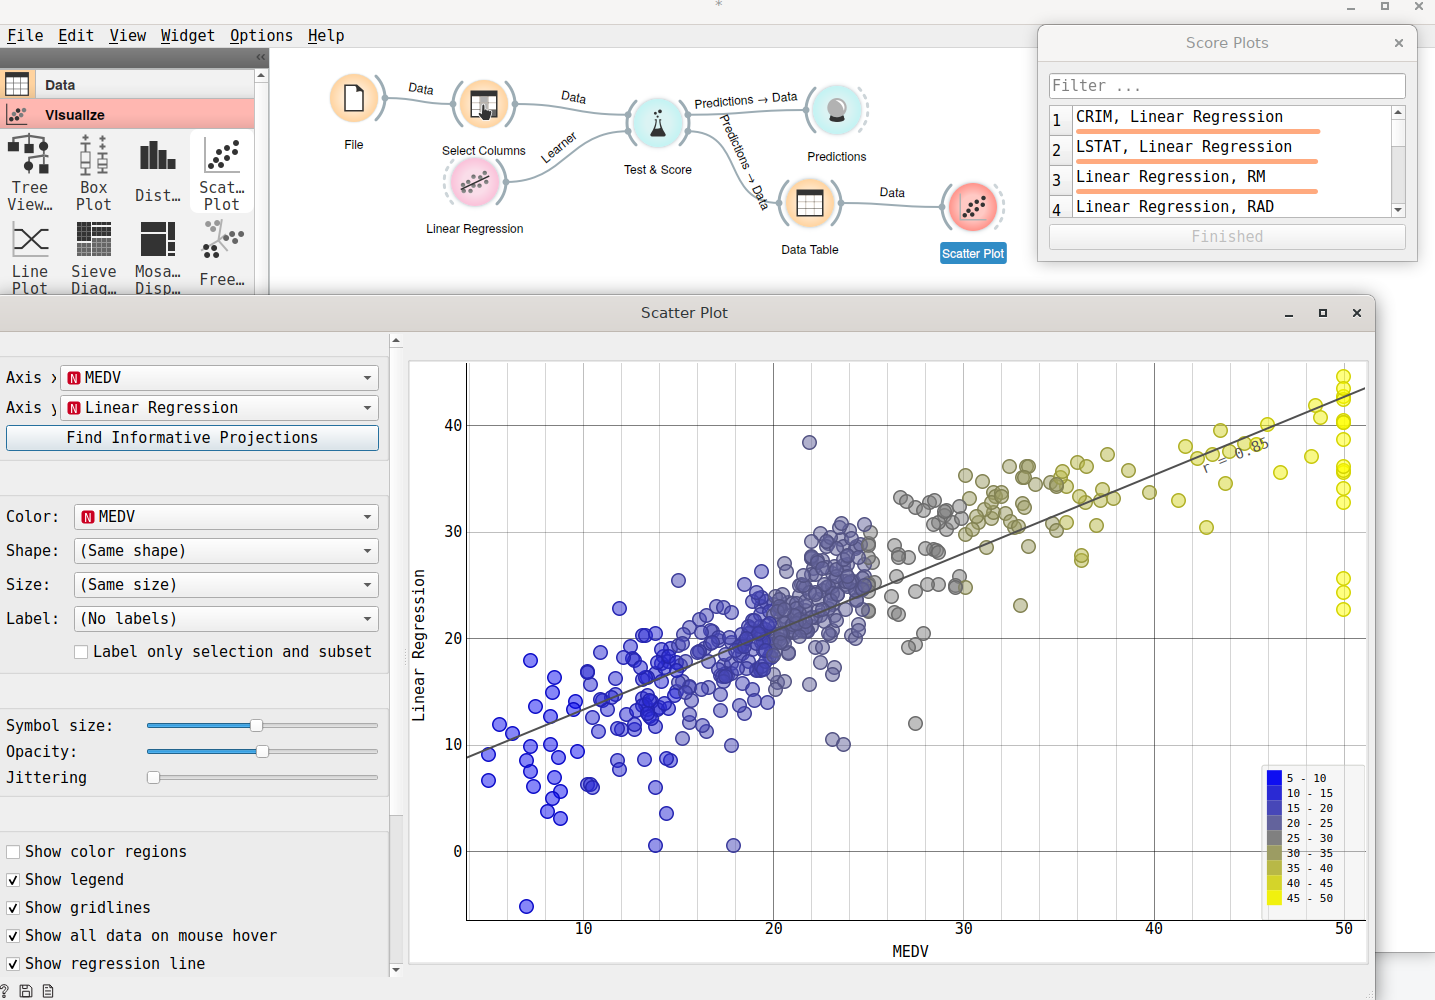
\includegraphics[scale=0.2]{ris_04.png}

\end{frame}


\begin{frame}{Полиноминальная регрессия}

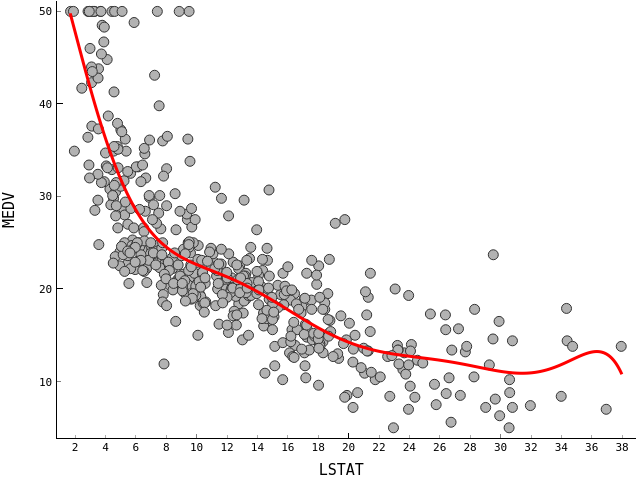
\includegraphics[scale=0.5]{ris_05.png}

Построено по таблице housing.tab, входит в базовый набор таблиц Orange3.
\end{frame}


\section{Понижение размерности.}

\begin{frame}
Отбор признаков. Выявление избыточных признаков с помощью фильтров.  Выделение признаков. 
Анализ главных компонент. Ограничения РСА. 
Применение оберток для задания модели вопросов о признаках. Другие методы обработки признаков.


Многомерное шкалирование.
\end{frame}


\begin{frame}{Отбор признаков}

Отбор признаков, известный также как отбор переменных, отбор атрибутов или отбор поднабора переменных, это процесс отбора подмножества значимых признаков (переменных зависимых и независимых) для использования в построении модели. Техники отбора признаков используются по четырём причинам:
\begin{itemize}


  \item упрощение моделей для того, чтобы сделать их проще для интерпретации исследователями/пользователями,
   \item    более короткое время тренировки,
   \item    чтобы избежать проклятие размерности,
   \item    улучшенное обобщение путём сокращения переобучения.
\end{itemize}
\end{frame}


\begin{frame}{Отбор признаков}
Центральный посыл использования техники отбора признаков — что данные содержат некоторые признаки, которые либо излишни, либо не значимы, а потому могут быть удалены без существенной потери информации. Излишни и не значимы являются двумя различными понятиями, поскольку один значимый признак может быть излишним при присутствии другого существенного признака, с которым он сильно коррелирует


\end{frame}





\begin{frame}{Снижение размерности. Важные моменты}
\begin{itemize}
  \item  Переменные, значения которых можно измерять в эксперименте, имеют для исследуемого объекта или явления нередко достаточно условный характер, лишь опосредовано 
  отражая его внутреннюю структуру, движущие силы (механизмы) или действующие на объект факторы. 
  
  \item Когда неизвестный фактор проявляется в изменении нескольких переменных, в процессе анализа можно наблюдать существенную корреляцию или связь между этими 
  переменными. 
  Тем самым глубинных (скрытых, латентных) факторов может быть существенно меньше, чем измеряемых переменных, даже само число которых выбирается исследователем достаточно 
  субъективно.
\end{itemize} 
 \end{frame}
 
   
\begin{frame}{Снижение размерности. Важные моменты}
\begin{itemize}
  
  
  \item Степень влияния фактора на некоторый показатель (переменную) проявляется в величине дисперсии (в разбросе или диапазоне изменения значений) этого показателя при 
  изменении значений фактора.    Действительно, изменение более мощного фактора будет приводить к большим изменениям показателя, на который он оказывает влияние.

\end{itemize} 
 \end{frame}
 
   
\begin{frame}{Снижение размерности.Важные моменты}
\begin{itemize}

  
  \item Если расположить оси исходных переменных ортогонально друг к другу (что также является определенным субъективным произволом, поскольку многие переменные связаны, коррелированы между собой, т. е. не могут считаться независимыми или ортогональными друг к другу), то можно обнаружить, что в этом (многомерном) пространстве объекты группируются (в соответствии со своими координатами) в виде некоторого облака или эллипсоида рассеяния, более вытянутого в одних направлениях и почти плоского в других.
  
  \end{itemize} 
 \end{frame}
 
   
\begin{frame}{Снижение размерности. Важные моменты}
\begin{itemize}

   \item   Если теперь провести новые оси координат соответственно осям такого эллипса рассеяния, то можно говорить о выделении так называемых факторов, более важных и существенных для изучаемого феномена по сравнению с исходными переменными, и оценивать сравнительную значимость этих факторов в смысле их влияния на дисперсию объектов. При этом обычно оказывается, что толщина такого облака рассеяния по некоторым осям настолько мала, что эти оси (малозначимые факторы) можно в дальнейшем вовсе исключить из рассмотрения. Это означает, что нам удалось снизить размерность исходного пространства переменных.  

\end{itemize} 
 \end{frame}
 
 
 \begin{frame}{Как работает метод главных компонент}
 


Для выбора первой оси  главной компоненты  нужно для каждой прямой посчитать сумму квадратов расстояний от всех точек до этой прямой и выбрать среди них ту, для которой эта сумма квадратов будет минимальной. Это похоже на поиск регрессионной прямой: разница состоит в том, что когда мы искали регрессионную прямую, мы считали расстояние «по вертикали», а сейчас считаем обычное расстояние от точки до прямой (вдоль направления, вертикального к прямой). Конечно, всех возможных прямых очень много, но задача отыскания самой лучшей из них оказывается довольно простой: компьютеры с ней справляются очень эффективно даже для пространств высокой размерности. 
 \end{frame}

\begin{frame}{Снижение размерности.Пример}
  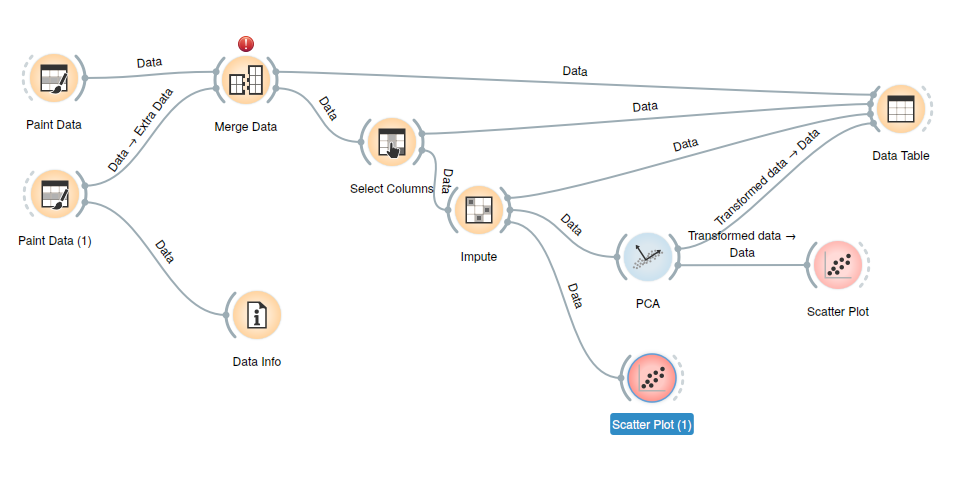
\includegraphics[scale=0.3]{task06_01.png}
\end{frame} 
 
 
 \begin{frame}{Метод фильтров}
    Методы фильтров выбирают переменные независимо от модели. Они базируются только на общих признаках, 
    таких как корреляция переменной с предсказанием. Методы фильтров подавляют наименее интересные переменные. 
    Другие переменные будут частью классификации или модели регрессии, использованной для классификации или предсказания.
 Эти методы очень эффективны по времени вычисления и устойчивы к переобучению. 
 \end{frame} 
 
 
 \begin{frame}{Метод фильтров}
  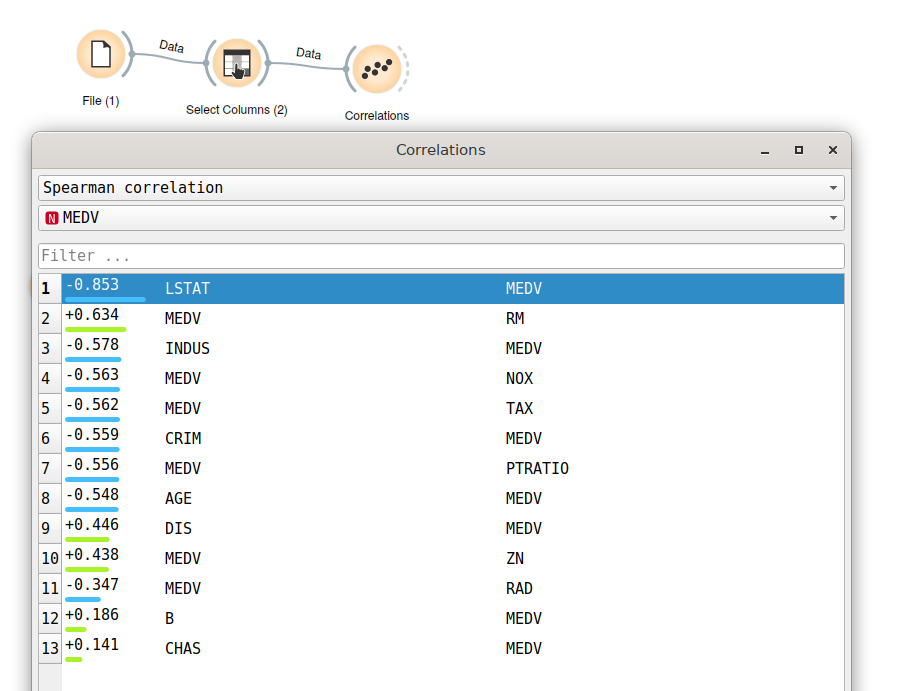
\includegraphics[scale=0.4]{task07_01.png}
 \end{frame} 
 
\begin{frame}{Применение оберток для задания модели вопросов о признаках}
  Методы обёртывания используют модель априорной оценки результата для оценки поднаборов признаков. Каждый новый поднабор используется для тренировки модели,
   которая проверяется на контрольной выборке. 
   На этой контрольной выборке считается число ошибок (показатель ошибок модели), которое даёт оценку для данного подмножества. Так 
   как методы обёртывания тренируют модель для каждого поднабора, они вычислительно очень затратны, но дают, как правило, лучший набор признаков для конкретного типа модели.
\end{frame}
 
  \begin{frame}{Метод оберток}
  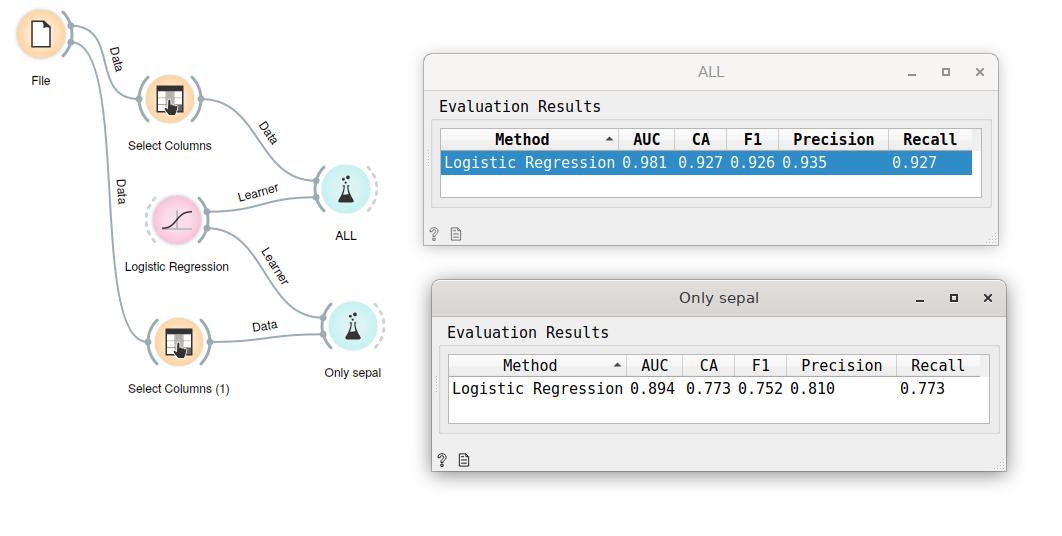
\includegraphics[scale=0.4]{task07_02.png}
 \end{frame} 
 
\begin{frame}{Метод вложения}

Метод вложения для отбора признаков
Методы вложения были предложены как попытка комбинации преимуществ двух предыдущих методов. 
Обучающий алгоритм имеет преимущество 
собственного процесса выбора переменной и осуществляет выбор признаков и классификацию одновременно. 
Метод вложения реализуется программно. 
\end{frame}




\section{Модель алгоритмов машинного обучения.}

\begin{frame}{Модель алгоритмов, метод обучения.}

Задано множество объектов X, множество допустимых ответов Y. 
Существуют пары <объект,ответ>,  которые будем  называть прецедентами. 
Совокупность  называется обучающей выборкой (training sample).



Задача обучения по прецедентам заключается в том, чтобы по  обучающей выборке 
восстановить зависимость, то есть построить решающую функцию  или алгоритм допускающий эффективную компьютерную 
реализацию.

\end{frame}  

\begin{frame}{Модель алгоритмов, метод обучения.}
В задачах обучения по прецедентам  пара <объект,ответ> 
это не реальные объекты, а лишь доступные данные о них. 
Данные могут быть неточными, поскольку измерения  свойств объектов и ответов обычно
выполняются с погрешностями. 

При это данные могут быть неполными, 
поскольку измеряются не все мыслимые признаки, а лишь физически доступные для измерения.
В результате одному и тому же описанию x могут соответствовать различные объекты и различные ответы. 
\end{frame}  

\begin{frame}{Модель алгоритмов, метод обучения.}

В таком случае   алгоритм или функция описывающие зависмость  не является функцией.
Устранить эту некорректность позволяет вероятностная постановка задачи.
Вместо существования неизвестной целевой зависимости можно считать что 
существует  неизвестное вероятностного распределения на множестве пар объектов и ответов
с плотностью p(x, y), из которого случайно и независимо выбираются  некоторое количество  наблюдений. 
Такие выборки называются простыми или случайными одинаково распределёнными.
Вероятностная постановка задачи считается более общей, так как функциональную зависимость можно 
представить в виде вероятностного распределения $p(x, y) = p(x)p(y|x)$, положив $p(y|x) = δ(y − y ∗ (x))$, где $\delta(z)$ — дельта-функция.

\end{frame}  



\begin{frame}{Основные виды классификаторов машинного обучения.}

Методы машинного обучения можно разделить на 3 основные категории: контролируемое, 
неконтролируемое и подкрепляемое обучение. Контролируемое или обучение с учителем  уже обсуждалось выше.

\end{frame}


\begin{frame}{Основные виды классификаторов машинного обучения.}
Контролируемое обучение полезно в тех случаях, когда свойство (ярлык) доступно для определенного массива данных (обучающего набора), но на данный момент оно отсутствует и должно быть предсказано для других случаев. 
\end{frame}


\begin{frame}{Основные виды классификаторов машинного обучения.}
Неконтролируемое обучение используется для обнаружения неявных отношений в данном немаркированном наборе данных. 

Формально:
Пусть X - множество объектов  - описаний некоторых
объектов. Необходимо найти множество  взаимосвязей этих объектов.
Качество выявления взаимосвязей проверяется некоторой метрикой,
выбранной исходя из решаемой задачи.

\end{frame}


\begin{frame}{Основные виды классификаторов машинного обучения.}


Обучение без учителя используется для решения следующих
типов задач:
1. Задача кластеризации.
2. Поиск правил ассоциации.
3. Сокращение размерности данных.
4. Визуализация данных.

\end{frame}



\begin{frame}{Основные виды классификаторов машинного обучения.}

Под задачей поиска правил ассоциаций подразумевается
выявление в признаковых описаниях объектов (исходных данных)
таких наборов и значений признаков, которые особенно часто
(неслучайно часто) встречаются в исходных данных. Если же
проводить аналогию с первой задачей, то каждое правило в данном
случае может быть представлено как кластер.

\end{frame}


\begin{frame}{Основные виды классификаторов машинного обучения.}


Задача сокращения размерности данных состоит в следующем.
Существует большой (значительно большой) объем признаковых
описаний объектов. Причем, этот объем обуславливается
внушительным количеством измерений признакового пространства.
Необходимо представить те же данные в пространстве меньшей
размерности, при этом минимизировав потери информации.
Группировка по кластерам как раз и будет одним из вариантов
решения проблемы.
\end{frame}


\begin{frame}{Основные виды классификаторов машинного обучения.}


Задача визуализации данных является по сути частным случаем
предыдущей: ее суть – представить исходные данные в отображаемом
пространстве, то есть пространстве размерности 2 или 3.
Как следует из описанного выше, обучение без учителя в какой-
то мере так или иначе сводится к кластеризации. Поэтому для оценки
качества обучения данным способом как правило используют
метрики качества кластеризации. Причем, при их выборе
учитывается, что эти метрики не должны зависеть от исходных

\end{frame}






\begin{frame}{Функция потерь и функционал качества.}

Функция потерь (loss function) — это неотрицательная функция $L (a, x)$,
характеризующая величину ошибки алгоритма a на объекте x. Если $L (a, x) = 0$,
то ответ $a(x)$ называется корректным.



\end{frame}


\begin{frame}{Функция потерь и функционал качества.}
$ L (a, x) = [a(x) + b = y^∗ (x)]$ - индикатор несовпадения с правильным ответом
(обычно применяется в задачах классификации);


$L (a, x) = |a(x) − y ∗ (x)| > \epsilon$  - индикатор существенного отклонения от пра-
вильного ответа, где $\epsilon$ - заданный порог точности.


\end{frame}

\begin{frame}{Функция потерь и функционал качества.}

Вообще, если L принимает только два значения 0 и 1, причём 1 соответствует ошибке,
 то функционал Q называется частотой ошибок алгоритма a на выборке X.

$L (a, x) = |a(x) − y^∗ (x)|$ — величина отклонения от правильного ответа; функ-
ционал Q называется средней ошибкой алгоритма a на выборке X ;

$L (a, x) = (a(x)−y^∗ (x))^2$ — квадрат отклонения от правильного ответа; функци-
онал Q называется средней квадратичной ошибкой алгоритма a на выборке X.

$L w (a, x) = w(x)L (a, x)$ — взвешенная функция потерь, где $w(x)$ — неотрица-
тельная весовая функция, характеризующая степень важности объекта x или
величину потери от ошибки на данном объекте; $L (a, x)$ — некоторая функция
потерь, например, любая из перечисленных выше.


\end{frame}




 
\begin{frame}{Принцип минимизации эмпирического риска.}

Эмпирическим риском называется средняя ошибка алгоритма на обучающей выборке. Метод минимизации эмпирического риска (empirical risk minimization, ERM) наиболее часто применяется для построения алгоритмов обучения. Он состоит в том, чтобы в рамках заданной модели выбрать алгоритм, имеющий минимальное значение средней ошибки на заданной обучающей выборке.

\end{frame}

\begin{frame}{Принцип минимизации эмпирического риска.}
С переобучением метода ERM связано два утверждения, которые на первый взгляд могут показаться парадоксальными.

Утверждение 1. Минимизация эмпирического риска не гарантирует, что вероятность ошибки на тестовых данных будет мала. Легко строится контрпример — абсурдный алгоритм обучения, который минимизирует эмпирический риск до нуля, но при этом абсолютно не способен обучаться. 

\end{frame}

\begin{frame}{Принцип минимизации эмпирического риска.}

Алгоритм состоит в следующем. Получив обучающую выборку, он запоминает её и строит функцию,
 которая сравнивает предъявляемый объект с запомненными обучающими объектами. 
 Если предъявляемый объект в точности совпадает с одним из обучающих, то эта функция 
 выдаёт для него запомненный правильный ответ. Иначе выдаётся произвольный ответ (например, случайный или всегда один и тот же). 
 Эмпирический риск алгоритма равен нулю, однако он не восстанавливает зависимость и не обладает никакой способностью к обобщению.

Вывод: для успешного обучения необходимо не только запоминать, но и обобщать.

\end{frame}

\begin{frame}{Принцип минимизации эмпирического риска.}


 Переобучение появляется именно вследствие минимизации эмпирического риска. Пусть задано конечное множество из D алгоритмов, 
которые допускают ошибки независимо и с одинаковой вероятностью. Число ошибок любого из этих алгоритмов 
на заданной обучающей выборке подчиняется одному и тому же биномиальному распределению.
 Минимум эмпирического риска — это случайная величина, равная минимуму из D 
 независимых одинаково распределённых биномиальных случайных величин. 
 Её ожидаемое значение уменьшается с ростом D. Соотвественно, с ростом D увеличивается 
 переобученность — разность вероятности ошибки и частоты ошибок на обучении.
 
\end{frame}

\begin{frame}{Принцип минимизации эмпирического риска.}

В данном модельном примере легко построить доверительный интервал переобученности, так как функция распределения минимума известна.
 Однако в реальной ситуации алгоритмы имеют различные вероятности ошибок, не являются независимыми,
  а множество алгоритмов, из которого выбирается лучший, может быть бесконечным.
   По этим причинам вывод количественных оценок переобученности является сложной задачей,
    которой занимается теория вычислительного обучения. До сих пор остаётся открытой 
    проблема сильной завышенности верхних оценок вероятности переобучения.
    
\end{frame}

\begin{frame}{Принцип минимизации эмпирического риска.}

Утверждение 3. Переобучение связано с избыточной сложностью используемой модели. Всегда существует оптимальное значение сложности модели, при котором переобучение минимально. 

\end{frame}

\begin{frame}{Обобщающая способность}

Обобщающая способность (generalization ability, generalization performance). Говорят, что алгоритм обучения обладает способностью к обобщению, если вероятность ошибки на тестовой выборке достаточно мала или хотя бы предсказуема, то есть не сильно отличается от ошибки на обучающей выборке. Обобщающая способность тесно связана с понятиями переобучения и недообучения.
\end{frame}

\begin{frame}{Обобщающая способность.}

Переобучение, переподгонка (overtraining, overfitting) — нежелательное явление, возникающее при решении задач обучения по прецедентам, когда вероятность ошибки обученного алгоритма на объектах тестовой выборки оказывается существенно выше, чем средняя ошибка на обучающей выборке. Переобучение возникает при использовании избыточно сложных моделей.

Недообучение — нежелательное явление, возникающее при решении задач обучения по прецедентам, когда алгоритм обучения не обеспечивает достаточно малой величины средней ошибки на обучающей выборке. Недообучение возникает при использовании недостаточно сложных моделей. 

\end{frame}

\begin{frame}{Скользящий контроль}

Скользящий контроль или кросс-проверка или кросс-валидация (cross-validation, CV) — процедура эмпирического оценивания обобщающей способности алгоритмов, 
обучаемых по прецедентам.

Фиксируется некоторое множество разбиений исходной выборки на две подвыборки: обучающую и контрольную. Для каждого разбиения выполняется 
настройка алгоритма по обучающей подвыборке, затем оценивается его средняя ошибка на объектах контрольной подвыборки.
Оценкой скользящего контроля называется средняя по всем разбиениям величина ошибки на контрольных подвыборках.

\end{frame}

\begin{frame}{Скользящий контроль}

Если выборка независима, то средняя ошибка скользящего контроля даёт несмещённую оценку вероятности ошибки. 
Это выгодно отличает её от средней ошибки на обучающей выборке, которая может оказаться смещённой 
(оптимистически заниженной) оценкой вероятности ошибки, что связано с явлением переобучения.

Скользящий контроль является стандартной методикой тестирования и сравнения алгоритмов классификации, регрессии и прогнозирования. 

\end{frame}


\begin{frame}{Основные виды}

\end{frame}




\begin{frame}{Логистическая регрессия}
Логистическая регрессия представляет собой мощный статистический способ прогнозирования вероятности возникновения 
некоторого события с одной или несколькими независимыми переменными.
 Логистическая регрессия определяет степень зависимости между категориальной зависимой и одной или несколькими 
 независимыми переменными путем использования логистической функции, являющейся аккумулятивным логистическим распределением. 

\end{frame}




\begin{frame}{Логистическая регрессия.Алгоритм}
Линейная регрессионная модель не всегда способна качественно предсказывать значения зависимой переменной. Выбирая для построения модели линейное уравнение, мы естественным 
образом не накладываем никаких ограничений на значения зависимой переменной. А такие ограничения могут быть существенными.

Например, при проектировании оптимальной длины шахты лифта в новом здании необходимо учесть, что эта длина не может превышать высоту здания вообще.
\end{frame}


\begin{frame}{Логистическая регрессия.Алгоритм}

Линейная регрессионная модель может дать результаты, несовместимые с реальностью. С целью решения данных проблем полезно изменить 
вид уравнения регрессии и подстроить его для решения конкретной задачи.

Вообще, логит регрессионная модель предназначена для решения задач предсказания 
значения непрерывной зависимой переменной, при условии, что эта зависимая переменная 
может принимать значения на интервале от 0 до 1.
\end{frame}

\begin{frame}{Логистическая регрессия. Сигмоид}

Сигмоид — это гладкая монотонная возрастающая нелинейная функция,
 имеющая форму буквы «S», которая часто применяется для «приближения» 
 значений некоторой величины к нулю и единице


$$  y=a_0 + a_1x_1+ a_2x_2 ...+a_nx_n $$

$$ f(y) = \frac{1}{1 + e^{-y}}$$



\end{frame}



\begin{frame}{Логистическая регрессия.Применение}

Данный алгоритм может быть использован для:
    \begin{itemize}

  \item оценки компартмента предприятия с использованием косвенных данных связи с другими предприятиями в прошлом объемы по типам продукции, регион и т.п.;
  \item измерении показателей успешности  тех или иных мер;
  \item предсказании доходов с определенного продукта;
    \end{itemize}
    

\end{frame}





\begin{frame}{Дерево принятия решений}

Дерево принятия решений — средство поддержки принятия решений, которое использует 
древовидный граф или модель принятия решений, а также возможные последствия их работы, 
включая вероятность наступления события, затраты ресурсов и полезность. 

\end{frame}


\begin{frame}{Дерево приннятия решения}

Деревья принятия решений и случайные леса

Один из самых распространeнных алгоритмов машинного обучения.
 Используется в статистике и анализе данных для прогнозных моделей. 
 Структура представляет собой "листья" и "ветки". 
 На "ветках" дерева решения записаны атрибуты, 
 от которых зависит целевая функция, в "листьях” записаны значения целевой функции, 
 а в остальных узлах – атрибуты, по которым различаются случаи.

\end{frame}


\begin{frame}{Дерево приннятия решения. Алгоритм}


Чтобы классифицировать новый случай, надо спуститься по дереву до листа и выдать соответствующее значение. 
Цель состоит в том, чтобы создать модель, которая предсказывает значение целевой 
переменной на основе нескольких входных переменных. Осуществляется перебор  столбцов.
\end{frame}

\begin{frame}{Дерево принятия решения. Пример}


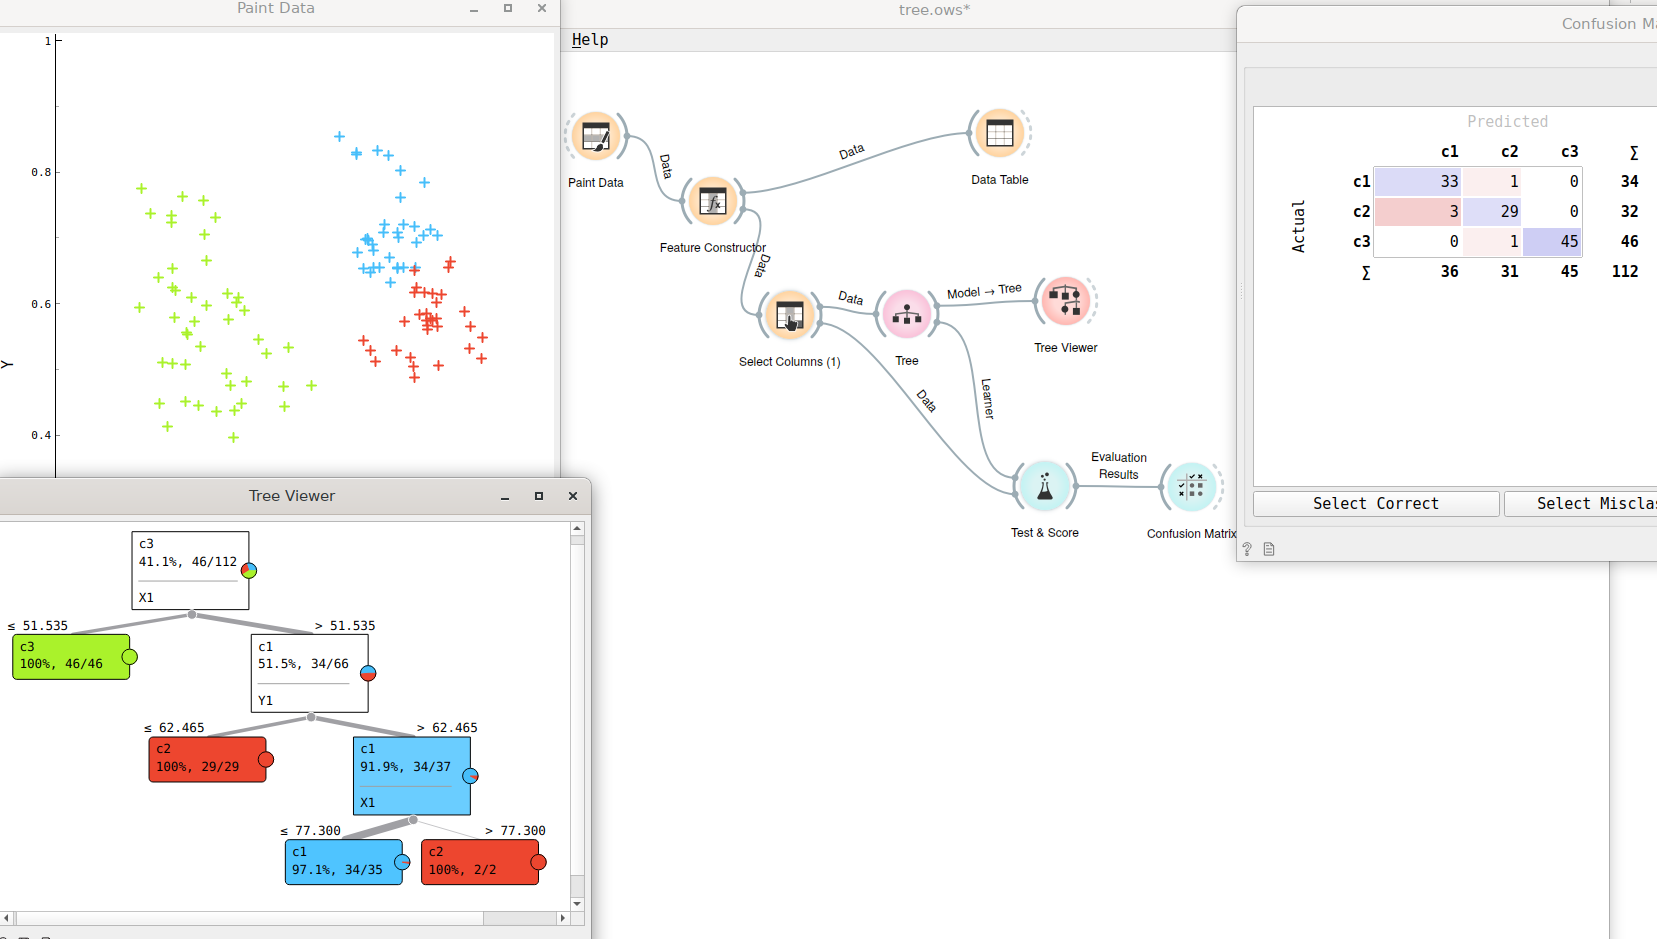
\includegraphics[scale=0.2]{task08_01.png}

\end{frame}


\begin{frame}{Дерево принятия решения. Пояснения}


\begin{textblock*}{120mm}(15mm,15mm)
 

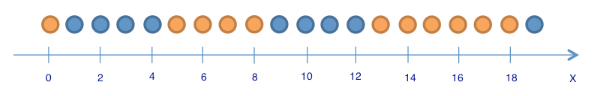
\includegraphics[scale=0.4]{ris_02.png}

\end{textblock*} 


\begin{textblock*}{90mm}(15mm,35mm)
Если мы наудачу вытащили шарик, 
то он с вероятностью $ p_1=\frac{9}{20} $ будет синим и с вероятностью $ p_2=\frac{11}{20} $ – желтым. 
Значит, энтропия состояния  $S_0=-\frac{9}{20}log_2{\frac{9}{20}}-\frac{11}{20}log_2{\frac{11}{20}} \approx 1$

Само это значение пока ни о чем нам не говорит. 
Как изменится энтропия, если разбить шарики на две группы – с координатой меньше либо равной 12 и больше 12?

$https://www.pvsm.ru/python/249240$
\end{textblock*} 


\end{frame}


\begin{frame}{Дерево принятия решения. Пояснения}

\begin{textblock*}{120mm}(15mm,15mm)

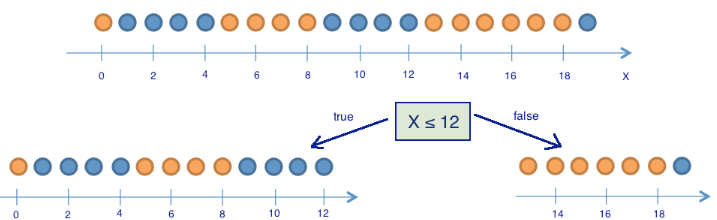
\includegraphics[scale=0.35]{ris_03.png}

\end{textblock*} 

\begin{textblock*}{90mm}(15mm,50mm)
В левой группе оказалось 13 шаров, из которых 8 синих и 5 желтых. 
Энтропия этой группы равна
 $S_1=-\frac{5}{13}log_2{\frac{5}{13}}-\frac{8}{13}log_2{\frac{8}{13}} \approx 0.96$. 
В правой группе оказалось 7 шаров, из которых 1 синий и 6 желтых. 
Энтропия правой группы равна 
$S_2=-\frac{1}{7}log_2{\frac{1}{7}}-\frac{6}{7}log_2{\frac{6}{7}} \approx 0.6$

$https://www.pvsm.ru/python/249240$
\end{textblock*} 


\end{frame}

\begin{frame}{Метод опорных векторов (SVM) }
Метод опорных векторов (SVM) — это набор алгоритмов, использующихся для задач классификации и регрессионного анализа. 
Учитывая, что в N-мерном пространстве каждый объект принадлежит одному из двух классов, SVM генерирует (N-1)-мерную 
гиперплоскость с целью разделения этих точек на 2 группы. Это как если бы вы на бумаге изобразили точки двух разных 
типов, которые можно линейно разделить. Помимо того, что метод выполняет сепарацию объектов, SVM подбирает 
гиперплоскость так, чтобы та характеризовалась максимальным удалением от ближайшего элемента каждой из групп.
\end{frame}


\begin{frame}{SVM. Пример}


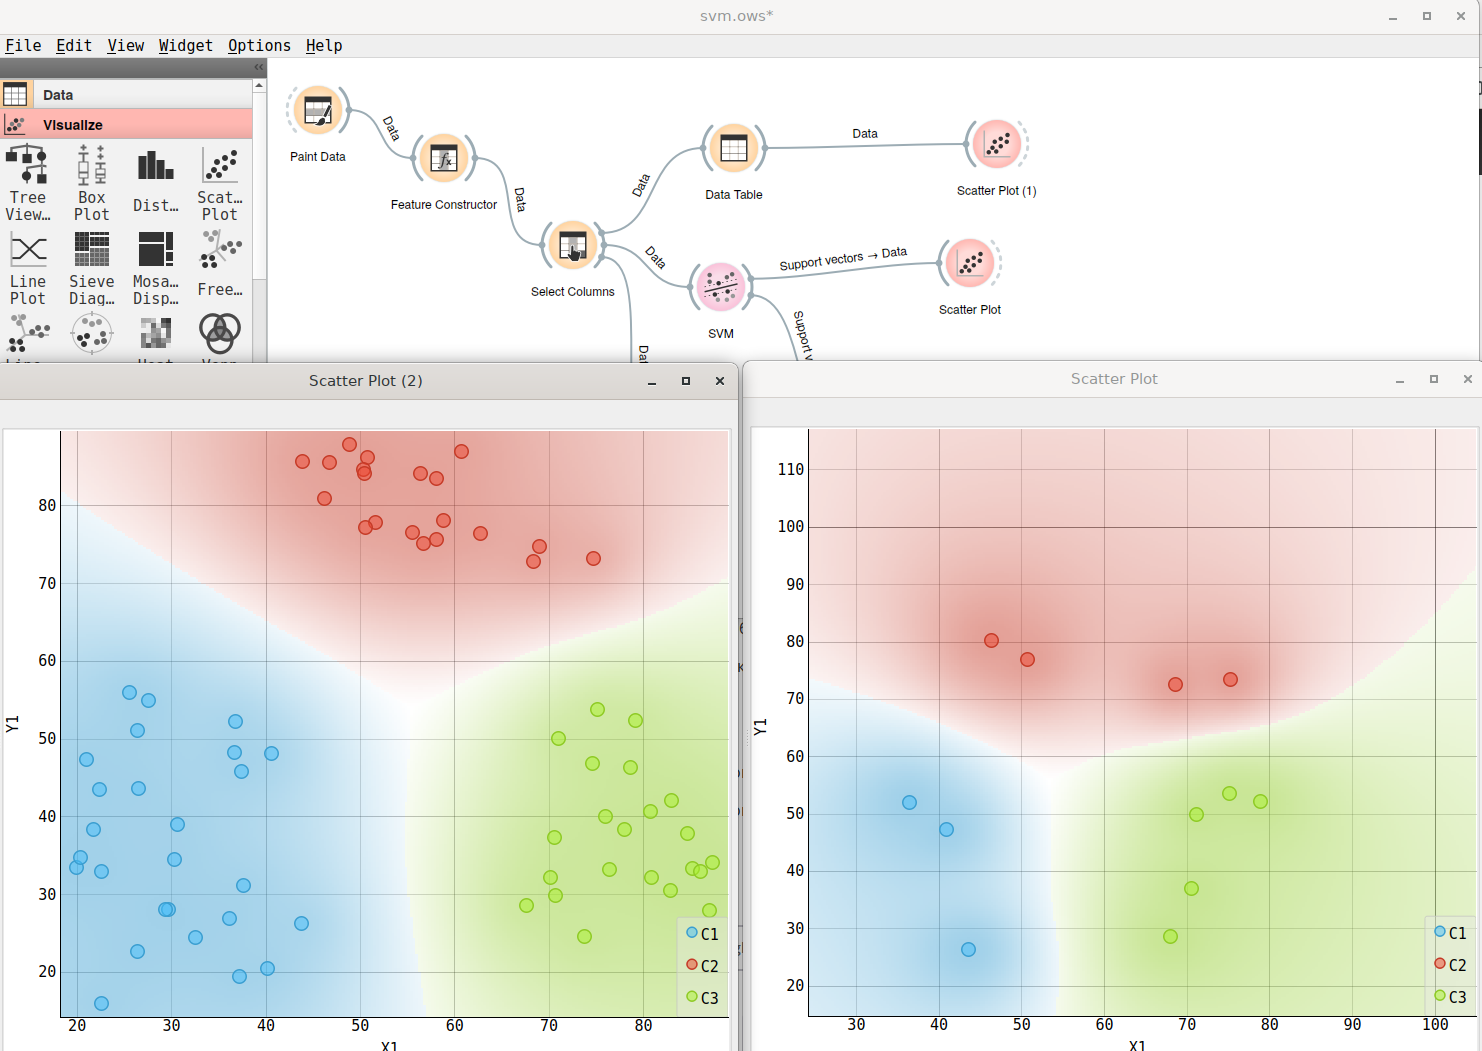
\includegraphics[scale=0.2]{task09_01.png}

\end{frame}

\begin{frame}{Метод ансамблей}

Метод ансамблей основан на обучающих алгоритмах, которые формируют множество классификаторов, а затем сегментируют 
новые точки данных, отталкиваясь от голосования или усреднения. 
Оригинальный метод ансамблей — не что иное, как Байесовское усреднение, но более поздние алгоритмы включают исправления ошибок выходного кодирования, бэггинг (bagging) и бустинг (boosting). 
\end{frame}


\begin{frame}{Метод ансамблей}

Бустинг направлен на превращение слабых моделей в сильные путем построения ансамбля классификаторов. 
Бэггинг также агрегирует усовершенствованные классификаторы, но используется при этом параллельное обучение 
базовых классификаторов. Бэггинг — улучшающее объединение, а бустинг — улучшающее пересечение.
\end{frame}


\begin{frame}{Random Forest}
Метод случайного леса (Random Forest) представляет собой дальнейшее улучшение бэггинга деревьев решений, 
которое заключается в устранении корреляции между деревьями. Как и в случае с бэггингом,
 мы строим несколько сотен деревьев решений по обучающим бутстреп-выборкам. 
 Однако на каждой итерации построения дерева случайным образом выбирается m из p подлежащих рассмотрению предикторов и разбиение разрешается выполнять только по одной из m этих переменных.
\end{frame}

\begin{frame}{Random Forest}
Смысл этой процедуры, оказавшейся весьма эффективной для повышения качества получаемых решений, заключается в том, что с вероятностью (p−m)/p
блокируется какой-нибудь потенциально доминирующий предиктор, стремящийся войти в каждое дерево. Если доминирование таких предикторов разрешить, то все деревья в итоге будут очень похожи друг на друга, а получаемые на их основе предсказания будут сильно коррелировать и снижение дисперсии будет не столь очевидным. Благодаря блокированию доминантов, другие предикторы получат свой шанс, и вариация деревьев возрастает.
\end{frame}

\begin{frame}{Random Forest}
Выбор малого значения m при построении случайного леса обычно будет полезным при наличии большого числа коррелирующих предикторов. Естественно, если случайный лес строится с использованием m=p, то вся процедура сводится к простому бэггингу.
\end{frame}


\begin{frame}{ROC -кривая}
Часто результат работы алгоритма на фиксированной 
тестовой выборке визуализируют с помощью ROC-кривой 
(ROC = receiver operating characteristic, 
иногда говорят «кривая ошибок»), а качество оценивают как площадь 
под этой кривой – AUC (AUC = area under the curve).
$https://dyakonov.org/$ и далее

\end{frame}
\begin{table}[tab:roccurve]
\caption{Таблица для построения ROC-кривой}
\label{tab:my-table}
\resizebox{\textwidth}{!}{%
\begin{tabular}{|c|c|}
\hline
Оценка логистической регрессии & класс \\ \hline
0.6 & 1 \\ \hline
0.5 & 1 \\ \hline
0.4 & 1 \\ \hline
0.2 & 0 \\ \hline
0.2 & 1 \\ \hline
0.1 & 0 \\ \hline
\end{tabular}%
}
\end{table}

\begin{frame}{ROC -кривая}

Чтобы нарисовать ROC-кривую  нужно координатную плоскость, разбить на m равных частей горизонтальными линиями 
и на n – вертикальными, где m – число 1 среди правильных меток теста (в нашем примере m=3), n – число нулей (n=4). 
В результате квадрат разбивается сеткой на m×n блоков.
\end{frame}


\begin{frame}{ROC -кривая}

Теперь будем просматривать строки таблицы сверху вниз и прорисовывать на сетке линии, переходя их одного узла в другой.
 Стартуем из точки (0, 0). 
 Если значение метки класса в просматриваемой строке 1, то делаем шаг вверх; если 0, то делаем шаг вправо. 
 Ясно, что в итоге мы попадём в точку (1, 1), т.к. сделаем в сумме m шагов вверх и n шагов вправо.

\end{frame}


\begin{frame}{ROC -кривая}

Если у нескольких объектов значения оценок равны, 
то мы делаем шаг в точку, которая на a блоков выше и b блоков правее(по диагонали), 
в нашем случае  4 и 5 строки имеют один и тот же  результат логистической регресии,
 поэтому будет сдвиг  по диагонали
В частности, если все объекты 
имеют одинаковую метку, то мы сразу шагаем из точки (0, 0) в точку (1, 1).


\end{frame}


%\begin{frame}
%  \frametitle{чсчс}
%  \framesubtitle{чсчсчссчч}
%\begin{block}{}
%\begin{columns}
%  \begin{column}{.5\textwidth}
%fgsdf
%  \end{column}
%  \begin{column}{.5\textwidth}
%ававаава
%  \end{column}
%\end{columns}
%\end{block}

%\begin{block}{}
%\begin{columns}
%  \begin{column}{.5\textwidth}
%scxcsc
%  \end{column}
%  \begin{column}{.5\textwidth}
%ававаава
%  \end{column}
%\end{columns}
%\end{block}


%\end{frame}



\end{document}
